% 2011 年浙江卷理科第 20 题：三棱锥 P-ABC，O 在 AD 上，PO⊥平面 ABC。
% 来源 PDF：普通高考/2011/2011浙江理.pdf，SHA-256 0239778f574bc3ce6d7aca5024aa6333f80d131abaf699f79c46472394f8cd65。
% 原页：第 2 页第 1 栏，书页码 710。示意。
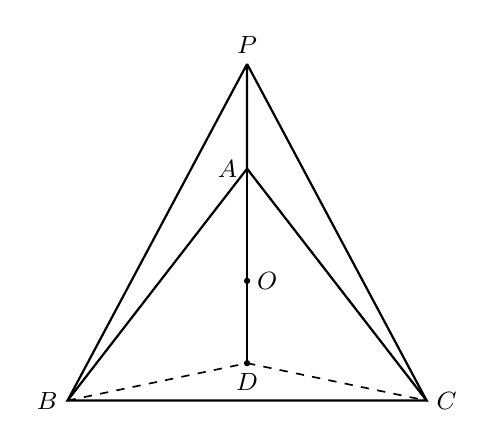
\begin{tikzpicture}[>=stealth, semithick, font=\small, scale=0.95]
  \coordinate (D) at (0,0);
  \coordinate (B) at (-2.4,-0.5);
  \coordinate (C) at (2.4,-0.5);
  \coordinate (A) at (0,2.6);
  \coordinate (O) at (0,1.1);
  \coordinate (P) at (0,4.0);
  \draw[thick] (A)--(B)--(C)--cycle;
  \draw[thick] (P)--(A) (P)--(B) (P)--(C);
  \draw[dashed] (A)--(C);
  \draw[dashed] (P)--(O);
  \draw[dashed] (B)--(D);
  \draw[dashed] (D)--(C);
  \draw (A)--(D);
  \fill (D) circle (1.2pt) node[below] {$D$};
  \fill (O) circle (1.2pt) node[right] {$O$};
  \node[left] at (A) {$A$};
  \node[left] at (B) {$B$};
  \node[right] at (C) {$C$};
  \node[above] at (P) {$P$};
\end{tikzpicture}
